%%
%% Copyright (C) 2008  Distributed Computing System (DCS) Group, Computer
%% Science Department - University of Piemonte Orientale, Alessandria (Italy).
%%
%% This program is free software: you can redistribute it and/or modify
%% it under the terms of the GNU Lesser General Public License as published
%% by the Free Software Foundation, either version 3 of the License, or
%% (at your option) any later version.
%%
%% This program is distributed in the hope that it will be useful,
%% but WITHOUT ANY WARRANTY; without even the implied warranty of
%% MERCHANTABILITY or FITNESS FOR A PARTICULAR PURPOSE.  See the
%% GNU Lesser General Public License for more details.
%%
%% You should have received a copy of the GNU Lesser General Public License
%% along with this program.  If not, see <http://www.gnu.org/licenses/>.
%%

%%
%% DcsShareGridBlender User Guide
%%
%% Author: Marco Guazzone, <marco.guazzone@gmail.com>
%%

\documentclass[italian,a4paper,12pt,titlepage,final]{article} 

%%@{ document preamble

%\usepackage{fancyhdr}
%\usepackage[headings]{fullpage}
\usepackage{amsmath}
\usepackage{amssymb}
\usepackage{amsthm}
\usepackage{babel}
\usepackage{color}
\definecolor{darkblue}{cmyk}{0.83,0.89,0.0,0.43}
\usepackage[T1]{fontenc}
\usepackage{framed}
\usepackage[headings]{fullpage}
\usepackage{graphicx}
%\usepackage[colorlinks,linkcolor=black,urlcolor=black,citecolor=black,hyperindex,plainpages=false]{hyperref} % Print Version
\usepackage[colorlinks,linkcolor=darkblue,urlcolor=blue,citecolor=darkblue,hyperindex,plainpages=false]{hyperref} % Electronic Version
\usepackage[latin1]{inputenc}
\usepackage{longtable}
\usepackage{multirow}
\usepackage{palatino}
\usepackage{setspace}
\usepackage{verbatim}

\makeatletter

\ifx\pdfoutput\defined
\hypersetup{
	pdftitle={DCS Grid Blender Submitter},
	pdfauthor={Marco Guazzone},
	pdfsubject={Sistemi Distribuiti e Grid Computing},
	pdfkeywords={Sistemi Distribuiti, Grid Computing, Scheduling, Rendering, Blender},
	pdfstartview={FitH}
}
\fi

\onehalfspacing % spacing to 1.5pt

%\newcommand{\mgTheApp}[1]{\emph{DcsShareGridBlender{#1}}
\newcommand{\mgTheApp}{\emph{DcsShareGridBlender}}
\newcommand{\mgTheAppFile}[1]{\emph{DcsShareGridBlender{#1}}}

\newcommand{\mgCode}[1]{\texttt{#1}}

%%@{ Custom environments
\newenvironment{mgComment}{\textcolor[gray]{0.8}\bgroup}{\egroup}%
\newenvironment{mgLinkBox}{\begin{table}\begin{framed}}{\end{framed}\end{table}}%
\newenvironment{mgCodeBox}
{
\begin{quote}
\normalfont\ttfamily}%
{\end{quote}}

%%{\begin{framed}\begin{list}{}{
%{\begin{list}{}{
%%{\begin{framed}{
%%\setlength{\rightmargin}{\leftmargin}
%\setlength{\listparindent}{0pt}% needed for AMS classes
%\raggedright
%\setlength{\itemsep}{0pt}
%\setlength{\parsep}{0pt}
%\normalfont\ttfamily}%
%%\item[]}
%\item[]\begin{framed}\item[]}
%%}
%{\end{framed}\end{list}}%
%%{\end{list}\end{framed}}%
%%{\end{framed}}%
\newenvironment{mgWarnBox}[1]{\begin{table}\begin{framed}\par\textbf{#1}\newline\newline}{\end{framed}\end{table}}%
\newenvironment{mgToDo}{\begin{framed}\color{blue}}{\color{black}\end{framed}}%
\newenvironment{mgFixMe}{\begin{framed}\color{red}}{\color{black}\end{framed}}%
\newenvironment{mgDeprecated}{\begin{framed}\color{brown}}{\color{black}\end{framed}}%
%%@} Custom environments

\makeatother

%%@} document preamble

%%@{ document body

\begin{document}

\bibliographystyle{plain}

\title{\textbf{DCS ShareGrid Blender v. 1.0.2}\\
\ \\
Manuale Utente}

\author{
\begin{tabular}{cc}
Distributed System Computing Group & TOP-IX \tabularnewline
Universit\`a del Piemonte Orientale & TOrino Piemonte Internet eXchange \tabularnewline
(\href{http://dcs.di.unipmn.it}{http://dcs.di.unipmn.it}) & (\href{http://www.topix.it}{http://www.topix.it}) \tabularnewline
\end{tabular}}

\maketitle

\thispagestyle{empty}
\setcounter{page}{1}
\pagenumbering{roman}
\tableofcontents
%\listoffigures
\newpage

\pagenumbering{arabic}
\setcounter{page}{1}
\pagestyle{empty}

%%%%%%%%%%%%%%%%%%%%%%%%%%%%%%%%%%%%%%%%%%%%%%%%%%%%%%%%%%%%%%%%%%%%%%%%%%%%%%%%

\pagestyle{plain}

%%
%% Copyright (C) 2008  Distributed Computing System (DCS) Group, Computer
%% Science Department - University of Piemonte Orientale, Alessandria (Italy).
%%
%% This program is free software: you can redistribute it and/or modify
%% it under the terms of the GNU Lesser General Public License as published
%% by the Free Software Foundation, either version 3 of the License, or
%% (at your option) any later version.
%%
%% This program is distributed in the hope that it will be useful,
%% but WITHOUT ANY WARRANTY; without even the implied warranty of
%% MERCHANTABILITY or FITNESS FOR A PARTICULAR PURPOSE.  See the
%% GNU Lesser General Public License for more details.
%%
%% You should have received a copy of the GNU Lesser General Public License
%% along with this program.  If not, see <http://www.gnu.org/licenses/>.
%%

\section{Introduzione} \label{sec:intro}

Questa sezione, ha lo scopo di far comprendere all'utente i principi che stanno alla base del funzionamento dell'applicazione \mgTheApp{}; prima di addentrarsi in tale descrizione, verranno forniti alcuni cenni sul ``rendering'' e sul ``Grid computing''.

Nella sezione \S \ref{ssec:intro-render} si illustrano alcune delle problematiche riguardanti il ``rendering'' di immagini e di scene computerizzate; in \S \ref{ssec:intro-grid}, invece, si presenta, brevemente, l'idea che sta alla base del ``Grid computing''; infine, in \S \ref{ssec:intro-theapp} si illustra il funzionamento ad alto livello dell'applicazione \mgTheApp{}.

\subsection{Rendering} \label{ssec:intro-render}

Il \emph{rendering} di immagini o di sequenze di fotogrammi (\emph{frame}) consiste nell'applicare a un modello matematico (tipicamente rappresentato sottoforma di un modello \emph{wire-frame}) una serie di attributi statici o dinamici (come ``texture'', luci, ``bump mapping'', ...) con il fine di ottenere un'immagine o un'animazione completa di dettagli.

Si tratta di un'attivit\`a molto onerosa dal punto di vista computazionale: anche con la tecnologia attuale, il ``rendering'' di animazioni della durata di alcuni minuti pu\`o richiedere diverse ore di computazione, in modo particolare quando tali animazioni includono molti dettagli realistici.

La produzione di animazioni computerizzate e di immagini digitali di elevata qualit\`a, arricchite di dettagli realistici, \`e un'attivit\`a che evolve continuamente, grazie alle innovazioni tecnologiche e ai progressi delle tecniche grafiche.
Mentre, al giorno d'oggi, si \`e in grado di ottenere immagini e animazioni computerizzate che fino a qualche anno fa era impensabile produrre in un tempo relativamente breve, la domanda di potenza computazionale e di capacit\`a di memorizzazione non si \`e arrestata:
\begin{itemize}
\item una maggiore potenza computazionale \`e indispensabile per poter ottenere prodotti grafici di elevata qualit\`a in un tempo sempre pi\`u breve;
\item una maggiore capacit\`a di memorizzazione \`e necessaria in quanto l'aumento della qualit\`a dei dettagli delle immagini ha portato a ottenere prodotti grafici di dimensioni anche dell'ordine dei Gigabyte;
\item una maggiore velocit\`a di accesso ai dispositivi di memorizzazione \`e indispensabile a causa del trasferimento di enormi quantit\`a di dati.
\end{itemize}
Inoltre, mentre le innovazioni tecnologiche permettono la realizzazione di prodotti grafici di qualit\`a superiore, la maggiore accessibilit\`a, da parte degli esperti del settore, a risorse hardware potenti e a software professionali rende il settore della grafica computerizzata sempre pi\`u competitivo:
\begin{itemize}
\item macchine che fino a una decina di anni fa avrebbero richiesto forti investimenti finanziari oggi sono acquistabili a un prezzo relativamente basso;
\item software per la grafica professionale sono ora disponibili a prezzi accessibili o sono addirittura gratuiti.
\end{itemize}
L'applicazione \emph{Blender} \footnote{\href{http://www.blender.org}{http://www.blender.org}} \`e un esempio di software gratuito dotato di funzionalit\`a avanzate, mentre \emph{Elephant Dream} \footnote{\href{http://www.elephantdream.org}{http://www.elephantdream.org}} \`e il primo film di animazione 3D, disponibile gratuitamente, realizzato con un software gratuito come Blender \footnote{Attualmente, altri due film, \emph{Plum\'iferos} (\href{http://www.plumiferos.com}{http://www.plumiferos.com}), rilasciato a breve, e \emph{Peach} (\href{http://peach.blender.org}{http://peach.blender.org}), la cui produzione inizia a Ottobre, utilizzano il software Blender.}.

La soluzione comunemente adottata dai professionisti del settore, per la riduzione dei tempi di produzione, \`e l'utilizzo di un \emph{render-farm} (o \emph{render-wall}), ossia di un gruppo di macchine interconnesse (tipicamente, un ``cluster'') ottimizzate per le operazioni di ``rendering'': i tempi di produzione vengono accorciati attraverso una parallelizzazione del processo di ``rendering'' delle immagini o dei filmati.
In un'articolo apparso sulla rivista \emph{Byte and Switch}, si dice che la \emph{Pixar} avrebbe impiegato pi\`u di $2000$ anni per effettuare il ``rendering'' del film \emph{Cars} se avesse avuto a disposizione un singolo computer, mentre, grazie all'utilizzo di un ``render-farm'', il tutto \`e stato effettuato in soli $5$ anni \cite{ByteAndSwitch2006Pixar}.

L'utilizzo di un ``render-farm'' \`e possibile grazie al fatto che il ``rendering'' di immagini e di animazioni \`e un'attivit\`a altamente parallelizzabile: ogni ``frame'', o gruppo di ``frame'', di un'animazione pu\`o essere processato in modo separato e indipendente dagli altri, inviandolo su una delle macchine del ``render-farm''; in questo modo pi\`u ``frame'' di una stessa animazione possono essere processati contemporaneamente in parallelo su macchine differenti del ``render-farm'', attuando quindi una forma di ``rendering'' pseudo-parallelo. In maniera simile, un'immagine, pu\`o essere scomposta in una serie di mattonelle (\emph{tile}), ognuna delle quali pu\`o essere processata su una differente macchina del ``render-farm''.

Tipicamente, un ``render-farm'' \`e coordinato da un \emph{queue manager} il cui compito principale \`e la gestione dell'accodamento delle immagini e delle animazioni da sottoporre al ``rendering'' e la distribuzione dei relativi ``tile'' o ``frame'' sui computer facenti parte del ``render-farm'', per effettuarne il processamento. Un ``queue-manager'' abbastanza diffuso e disponibile gratuitamente \`e \emph{Dr. Queue} \footnote{\href{http://drqueue.org/cwebsite/}{http://drqueue.org/cwebsite/}}.

Malgrado l'utilizzo di un ``render-farm'' permetta di ridurre drasticamente i tempi di produzione, gli investimenti monetari richiesti per il suo acquisto e la relativa manutenzione sono in generale elevati e non sono sempre accompagnati da un immediato ritorno economico.

\subsection{Grid computing} \label{ssec:intro-grid}

L'avvento del \emph{Grid computing}, come paradigma di computazione, e l'emergere di \emph{sistemi Grid}, che sfruttano tale paradigma, ha reso possibile disporre di una elevata potenza computazionale e una grande capacit\`a di memorizzazione a costi molto ridotti.
L'obiettivo del ``Grid computing'' consiste nel permettere la condivisione, in modo coordinato e distribuito, di risorse eterogenee (tipicamente, computazionali o di memorizzazione) appartenenti a diverse entit\`a (individui o istituzioni), il tutto effettuato in modo trasparente rispetto a chi utilizza un sistema Grid \cite{Foster2001Anatomy}.

Detto in maniera pi\`u semplice, due o pi\`u comunit\`a (singoli utenti, universit\`a, aziende, etc.), anche separate da una larga distanza geografica, possono condividere, attraverso un sistema Grid, le rispettive risorse (di calcolo o di memorizzazione), in modo che gli utenti di ciascuna comunit\`a possano usare, in maniera del tutto trasparente (cio\`e, come se tutto avvenisse sulla propria macchina), le risorse che tutte le comunit\`a hanno messo a disposizione; le comunit\`a quindi hanno a disposizione una potenza computazionale maggiore di quella che avrebbero singolarmente, il tutto con un investimento economico pressoch\'e nullo.

Riguardo le singole propriet\`a di cui, la condivisione ottenuta tramite ``Grid computing'', deve godere, la condivisione distribuita permette, agli utenti del sistema, di utilizzare le varie risorse remote senza preoccuparsi della distanza geografica: le risorse possono essere poste anche a una distanza geografica molto vasta, come, ad esempio, quella su cui la rete Internet si estende.
Il coordinamento delle risorse condivise, invece, \`e necessario per poter interagire con risorse differenti tra loro e, in generale, indipendenti.
La trasparenza, permette agli utenti di un sistema Grid, per esempio, di non preoccuparsi di conoscere la locazione fisica di una certa risorsa (come un file o un programma) o di gestire problematiche derivanti dalla comunicazione di rete all'interno delle proprie applicazioni.

Oltre alle propriet\`a suddette, l'obiettivo del ``Grid computing'' \`e anche di quello di garantire che la condivisione sia sicura (ad es., privatezza, per chi sottomette delle computazioni, e integrit\`a, per chi mette a disposizione le proprie risorse per le computazioni) e che le risorse del sistema siano gestite nel modo pi\`u efficiente possibile.

Il componente di un sistema Grid che si occupa di raggiungere tali obiettivi prende il nome di \emph{middleware}; si tratta di uno strato software che si pone tra il sistema operativo e le applicazioni utente, composto da varie componenti, ognuno dei quali \`e preposto a uno specifico compito (ad es., gestione delle risorse, sicurezza, trasferimento di file, etc.).

Dato che il ``rendering'' di immagini o filmati digitali pu\`o, generalmente, essere scomposto in attivit\`a parallele e indipendenti, \`e possibile sfruttare il ``Grid computing'' per cercare di ridurre i tempi di produzione, in maniera simile a quanto avviene in un ``render-farm''.
I vantaggi che ne derivano comprendono:
\begin{itemize}
\item la riduzione dei tempi di produzione, grazie alla distribuzione del lavoro su diverse macchine;
\item l'abbattimento dei costi, grazie al risparmio sull'acquisto e sulla manutenzione di risorse hardware;
\item una maggiore affidabilit\`a, grazie alla risottomissione del lavoro su altre macchine del sistema, nel caso in cui alcune macchine diventino indisponibili.
\end{itemize}

\subsection{Applicazione \mgTheApp{}} \label{ssec:intro-theapp}

L'obiettivo dell'applicazione \mgTheApp{} \`e quello di sfruttare il ``Grid computing'' per effettuare il ``rendering'' di immagini e di animazioni di grafica computerizzata; attualmente \mgTheApp{} \`e in grado di supportare scene in formato \emph{Blender}.

L'idea di base di \mgTheApp{} \`e simile a quella utilizzata in un ``render-farm'': una scena viene logicamente divisa in gruppi contigui di ``frame'', ognuno dei quali viene processato su una delle macchine del sistema Grid, attualmente disponibili.
Per effettuare l'elaborazione di un certo gruppo di ``frame'' su una particolare macchina del sistema Grid, \mgTheApp{} trasferisce sulle macchine il file della scena insieme a eventuali risorse addizionali (come, ad esempio, delle texture).
Una volta che la computazione sulla macchina remota \`e terminata (ossia, il ``rendering'' di tutti i ``frame'' appartenenti al gruppo \`e stato completato), il risultato viene trasferito sulla macchina locale dell'utente.
Quando tutte le computazioni sono terminate, all'utente non rimane altro che assemblare i risultati ottenuti dal ``rendering'' dei vari gruppi di ``frame''.

Per effettuare tali operazioni, \mgTheApp{} interagisce con lo \emph{scheduler} del sistema Grid, cio\`e con quel componente software che si occupa di selezionare una macchina del sistema Grid e di assegnarle una certa computazione.

Il ruolo principale di \mgTheApp{} \`e, quindi, quello di fornire un'interfaccia ad alto livello tra l'utente, che intende effettuare il ``rendering'' di una scena Blender, e lo ``scheduler'' del sistema Grid. Per effettuare ci\`o, l'utente di \mgTheApp{} deve specificare le seguenti informazioni:
\begin{itemize}
\item \emph{Scene file}, il percorso completo del file della scena (file \mgCode{.blend}, in formato Blender);
\item \emph{Start frame}, il frame iniziale da cui far partire il ``rendering'' dell'intera scena; il valore di default \`e $1$.
\item \emph{End frame}, il frame finale in cui arrestare il ``rendering'' dell'intera scena; il valore di default \`e $1$.
\end{itemize}
L'utente pu\`o inoltre fornire altre informazioni, come:
\begin{itemize}
\item \emph{Scene name}, nome simbolico utilizzato per identificare la scena durante il processo di ``rendering''.
Se non viene specificato, viene costruito a partire dal nome dell'utente (ricavato dal sistema operativo) e dalla data corrente di sistema.
\item \emph{Scene step}, numero massimo di ``frame'' da assegnare a ogni gruppo in cui la scena viene logicamente divisa; pi\`u precisamente, se $F$ \`e il numero di ``frame'' da sottoporre al ``rendering'' e $S$ \`e il valore assunto da ``scene step'', la scena verr\`a logicamente partizionata in $\lceil F/S \rceil$ gruppi di ``frame'' contigui \footnote{L'operatore $\lceil x \rceil$ restituisce l'intero uguale o immediatamente superiore all'argomento $x$, cio\`e restituisce $x$, se $x$ \`e un numero intero, o la parte intera di $x$ incrementata di uno, se $x$ \`un numero reale con parte decimale non nulla.}, ciascuno contenente, al pi\`u, $S$ frame \footnote{Si noti che l'ultimo gruppo, cio\`e quello contenente l'ultimo ``frame'' della scena su cui effettuare il ``rendering'', potrebbe contenere un numero di ``frame'' inferiore a $S$; ci\`o capita quando $F$ non \`e un multiplo di $S$.}.
%L'operatore $\lceil x \rceil$ restituisce l'intero uguale o immediatamente superiore all'argomento $x$, cio\`e restituisce $x$, se $x$ \`e un numero intero, o la parte intera di $x$ incrementata di uno, se $x$ \`un numero reale.
Se tale informazione non viene fornita dall'utente, il valore di default usato da \mgTheApp{} \`e $25$.
\item \emph{Input file}, file, eventualmente compresso in formato ZIP, rappresentante una o pi\`u risorse aggiuntive, come, ad esempio, delle texture.
Se tale informazione non \`e fornita dall'utente, \mgTheApp{} suppone che la scena non abbia bisogno di alcuna risorsa addizionale.
\end{itemize}

La Fig.~\ref{fig:intro-workflow} fornisce una rappresentazione ad alto livello delle varie operazioni eseguite per effettuare il ``rendering'' di una scena tramite \mgTheApp{}.
Il numero che appare accanto alle frecce indica l'ordine temporale secondo cui avvengono le varie azioni:
\begin{enumerate}
\item L'utente crea un modello di una scena di animazione in Blender; in Fig.~\ref{fig:intro-workflow} si suppone che la scena sia composta da $300$ frame.
\item L'utente esegue l'applicazione \mgTheApp{}, inserendo, almeno, le seguenti informazioni:
\begin{itemize}
\item percorso completo al file della scena \mgCode{MyScene.blend};
\item numero del primo ``frame'' da cui far partire il ``rendering'' (in questo caso $1$);
\item numero dell'ultimo ``frame'' in cui far arrestare il ``rendering'' (in questo caso $300$).
\end{itemize}
Nella figura si ipotizza, anche, che l'utente specifichi esplicitamente che come ``step frame'' si utilizzi il valore $100$.
\item Quando l'utente richiede l'esecuzione del ``rendering'', l'applicazione \mgTheApp{}:
\begin{enumerate}
\item suddivide la scena in $300/100=3$ gruppi da $100$ ``frame'' contigui ciascuno: un gruppo per i ``frame'' da $1$ a $100$, uno per i ``frame'' da $101$ a $200$ e, infine, uno per i ``frame'' da $201$ a $300$;
\item contatta lo ``scheduler'' \emph{mygrid} del sistema \emph{ShareGrid};
\item invia allo ``scheduler'' le istruzioni per effettuare il ``rendering'' dei tre gruppi;
\item richiede allo ``scheduler'' l'esecuzione delle tre operazioni di ``rendering''.
\end{enumerate}
\item Lo ``scheduler'' provvede quindi a distribuire le operazioni di ``rendering'' sulle macchine di ShareGrid, non appena diventano disponibili; su ognuna di queste macchina avverr\`a l'effettivo processamento dei ``frame'' tramite Blender.
Occorre far notare che, da questo punto in poi, il ruolo principale di \mgTheApp{} \`e terminato; l'utente pu\`o infatti decidere di:
\begin{itemize} 
\item continuare a usare \mgTheApp{}, per monitorare lo stato di esecuzione del ``rendering'' o per sottomettere un nuovo ``rendering'';
\item usare l'interfaccia (testuale o grafica) dell'applicazione ``mygrid'' per monitorare lo stato di esecuzione del ``rendering'';
\item abbandonare la postazione di lavoro e controllare lo stato di esecuzione saltuariamente \footnote{L'applicazione ``mygrid'' deve per\`o rimanere in esecuzione sulla macchina dell'utente.}.
\end{itemize} 
\item A mano a mano che il ``rendering'' di ogni gruppo di ``frame'' termina, lo ``scheduler'' trasferisce il risultato sulla macchina dell'utente, nella stessa cartella da cui l'applicazione \mgTheApp{} \`e stata eseguita.
Per convenzione, il risultato di un ``rendering'' di un certo gruppo di ``frame'' \`e un file compresso in formato ZIP, il cui nome ha le seguente forma:
\begin{mgCodeBox}
$\langle$nome-file-scena$\rangle$-rendered.zip\_$\langle G_F \rangle$\_$\langle G_L \rangle$
\end{mgCodeBox} 
dove:
\begin{itemize}
\item $\langle$nome-file-scena$\rangle$ \`e il nome del file della scena, escluso il percorso e l'estensione;
\item $\langle G_F \rangle$ \`e il primo ``frame'' del gruppo da cui il ``rendering'' \`e iniziato;
\item $\langle G_L \rangle$ \`e l'ultimo ``frame'' del gruppo in cui il ``rendering'' \`e terminato.
\end{itemize}
Nel caso della figura, i file prodotti dalle tre operazioni di ``rendering'' sono:
\begin{mgCodeBox}
MyScene-rendered.zip\_$1$\_$100$ \newline
MyScene-rendered.zip\_$101$\_$200$ \newline
MyScene-rendered.zip\_$201$\_$300$
\end{mgCodeBox}
All'interno di ogni file compresso, il risultato del ``rendering'' (ad es., file in formato AVI) \`e contenuto dentro una cartella chiamata \emph{$\langle$nome-file-scena$\rangle$-rendered} (nel caso della figura, \emph{MyScene-rendered}).
\item Quando i ``rendering'' dei tre gruppi sono tutti terminati, l'utente pu\`o combinare in modo opportuno il contenuto dei tre file compressi.
\end{enumerate}

\begin{figure}
\centering
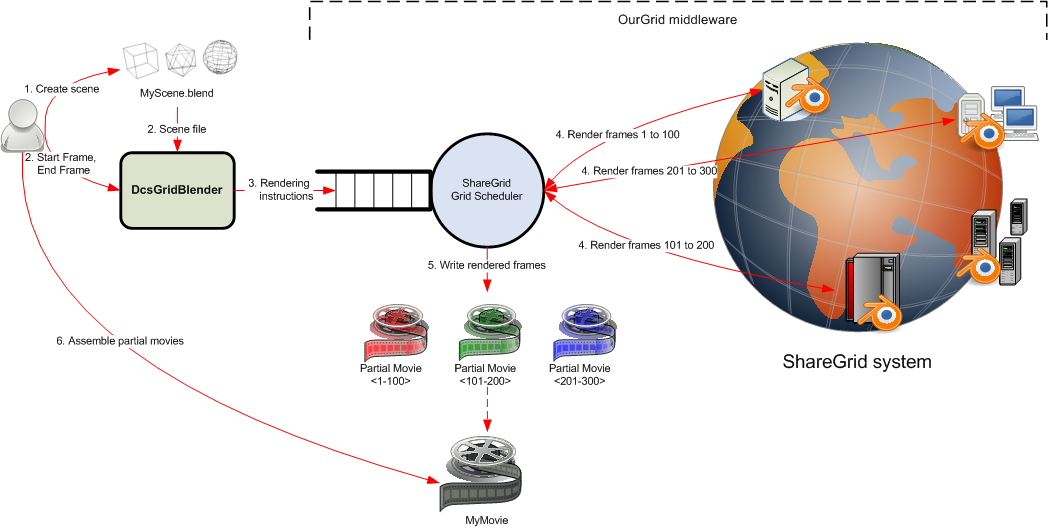
\includegraphics[scale=0.40]{images/DcsShareGridBlender_Block}
\caption{Workflow per il rendering di una scena tramite \mgTheApp{}.}
\label{fig:intro-workflow}
\end{figure}


%%
%% Copyright (C) 2008  Distributed Computing System (DCS) Group, Computer
%% Science Department - University of Piemonte Orientale, Alessandria (Italy).
%%
%% This program is free software: you can redistribute it and/or modify
%% it under the terms of the GNU Lesser General Public License as published
%% by the Free Software Foundation, either version 3 of the License, or
%% (at your option) any later version.
%%
%% This program is distributed in the hope that it will be useful,
%% but WITHOUT ANY WARRANTY; without even the implied warranty of
%% MERCHANTABILITY or FITNESS FOR A PARTICULAR PURPOSE.  See the
%% GNU Lesser General Public License for more details.
%%
%% You should have received a copy of the GNU Lesser General Public License
%% along with this program.  If not, see <http://www.gnu.org/licenses/>.
%%

\section{Installazione} \label{sec:inst}

Questa sezione descrive i passi necessari per installare l'applicazione \mgTheApp{}.

\subsection{Requisiti di Sistema} \label{ssec:inst-sysreq}

Per poter eseguire l'applicazione \mgTheApp{} \`e necessario che il proprio sistema disponga dei seguenti requisiti software:
\begin{itemize}
\item \emph{Java Runtime Environment} (\emph{JRE}) versione $1.6$, scaricabile, ad esempio, dal sito della \emph{Sun} (\href{http://java.sun.com}{http://java.sun.com}).
\item Componente \emph{mygrid} del middleware \emph{OurGrid}, versione $3.3.1$, scaricabile dal sito di \emph{OurGrid} (\href{http://www.ourgrid.org}{http://www.ourgrid.org}) e disponibile anche sul sito di \emph{ShareGrid} (\href{http://dcs.di.unipmn.it}{http://dcs.di.unipmn.it}).
\item Sistema operativo Unix-like, come, ad esempio, Linux (per soddisfare i requisiti del componente \emph{mygrid} di \emph{OurGrid}).
\item Programma in grado di scompattare file in formato \emph{ZIP}.
\end{itemize}

Per verificare che la versione del JRE installato nel proprio sistema sia quella corretta, eseguire, da un prompt dei comandi, il seguente comando:
\begin{mgCodeBox}
java -version
\end{mgCodeBox}
Dovrebbe apparire un messaggio mostrante la versione del JRE.
Per esempio, utilizzando il \emph{Sun JRE $1.6$ Update $2$}, il messaggio visualizzato, dopo l'esecuzione del comando precedentemente mostrato, dovrebbe essere simile al seguente:
\begin{mgCodeBox}
java version ``1.6.0\_02''\newline
Java(TM) SE Runtime Environment (build 1.6.0\_02-b05)\newline
Java HotSpot(TM) Client VM (build 1.6.0\_02-b05, mixed mode, sharing)
\end{mgCodeBox}

Per controllare che la versione del componente \emph{mygrid} del middleware \emph{OurGrid} sia quella richiesta, eseguire, da un prompt dei comandi, le seguenti istruzioni:
\begin{mgCodeBox}
cd /path/to/mygrid/installation\newline
./bin/mygrid version
\end{mgCodeBox}
Per esempio, nel caso in cui \emph{mygrid} sia stato scaricato dal sito di \emph{Sharegrid}, i comandi da eseguire sarebbero:
\begin{mgCodeBox}
cd shareGrid/clientSG\newline
./bin/mygrid version
\end{mgCodeBox}
L'output del comando dovrebbe essere simile al seguente:
\begin{mgCodeBox}
OurGrid 3.3.1 - MyGrid\newline
\newline
For MyGrid updates and additional information, see the\newline
OurGrid Project home page at http://www.ourgrid.org/ 
\end{mgCodeBox}

\`E inoltre indispensabile avere una connessione Internet per poter accedere all'infrastruttura Grid di \emph{ShareGrid}.

\subsection{Installazione} \label{sec:inst-inst}

Se i requisiti di sistema (\S \ref{ssec:inst-sysreq}) sono soddisfatti \`e possibile procedere all'installazione di \mgTheApp{}.
Al fine di semplificare la descrizione della procedura di installazione, nel seguito si effettueranno le seguenti assunzioni:
\begin{itemize}
\item L'utente ha installato il componente \emph{mygrid} attraverso il file e le istruzioni pubblicate sul sito di \emph{ShareGrid}; ne segue, che sul disco dell'utente \`e presente la cartella \emph{shareGrid}, creata durante il processo di installazione di \emph{mygrid}.
\item Il programma utilizzato dall'utente per scompattare i file in formato ZIP \`e \emph{unzip}.
\end{itemize}

Di seguito viene presentata la procedura di installazione di \mgTheApp{}.
\begin{enumerate}
\item Scaricare dal sito di \emph{ShareGrid} (\href{http://dcs.di.unipmn.it}{http://dcs.di.unipmn.it}) il file \mgTheAppFile{.zip}.
\item Scompattare il file all'interno della cartella \emph{shareGrid} creata durante l'installazione del componente \emph{mygrid}:
\begin{mgCodeBox}
cd shareGrid \newline
unzip \mgTheAppFile{.zip}
\end{mgCodeBox}
Se non si sono verificati errori, dovrebbe essere stata creata la cartella \mgTheApp{}.
\item Spostarsi nella directory \mgTheApp{}
\begin{mgCodeBox}
cd \mgTheApp{}
\end{mgCodeBox}
\item Eseguire lo script di installazione \emph{install.sh}
\begin{mgCodeBox}
./install.sh
\end{mgCodeBox}
\begin{enumerate}
\item Se l'esecuzione dello script termina con il messaggio:
\begin{mgCodeBox}
The path '/full/path/to/shareGrid/clientSG' seems to work! \newline
Installation succeded! \newline
Bye!!
\end{mgCodeBox}
allora \`e possibile proseguire con l'installazione.
\item Altrimenti, nel caso in cui venga mostrato il messaggio:
\begin{mgCodeBox}
!! WARNING !! \newline
MGROOT\_GUESS variable is set to a non existent path (\dots)! \newline
Please, set it to the MyGrid installation path. \newline
Installation failed. Sorry! \newline
Bye!!
\end{mgCodeBox}
editare il file \emph{install.sh} e impostare la variabile di ambiente \texttt{MGROOT\_GUESS} in modo che contenga il percorso completo della cartella in cui \`e stato installato il componente \emph{mygrid}. Per le assunzioni fatte in precedenza, tale percorso dovrebbe essere dato da \emph{/full/path/to/shareGrid/clientSG}: 
\begin{mgCodeBox}
MGROOT\_GUESS=/full/path/to/shareGrid/clientSG
\end{mgCodeBox}
Ripetere quindi il comando mostrato all'inizio di questo passo.
\end{enumerate}
\item Se l'esecuzione di \emph{install.sh} termina con successo, dovrebbe essere presente nella stessa cartella il nuovo file \mgTheAppFile{.sh}.
\item A questo punto, l'installazione di \mgTheApp{} \`e completata.
\end{enumerate}


%%
%% Copyright (C) 2008  Distributed Computing System (DCS) Group, Computer
%% Science Department - University of Piemonte Orientale, Alessandria (Italy).
%%
%% This program is free software: you can redistribute it and/or modify
%% it under the terms of the GNU Lesser General Public License as published
%% by the Free Software Foundation, either version 3 of the License, or
%% (at your option) any later version.
%%
%% This program is distributed in the hope that it will be useful,
%% but WITHOUT ANY WARRANTY; without even the implied warranty of
%% MERCHANTABILITY or FITNESS FOR A PARTICULAR PURPOSE.  See the
%% GNU Lesser General Public License for more details.
%%
%% You should have received a copy of the GNU Lesser General Public License
%% along with this program.  If not, see <http://www.gnu.org/licenses/>.
%%

\section{Esecuzione} \label{sec:exec}

In questa sezione verranno mostrati i passi base per effettuare il ``rendering'' di una semplice scena 3D tramite l'applicazione \mgTheApp{}.

Prima di eseguire l'applicazione \mgTheApp{}, assicurarsi che lo ``scheduler'' \emph{mygrid} sia in esecuzione; per maggiori dettagli su come eseguire ``mygrid'', si consulti la guida presente sul sito ufficiale di \emph{OurGrid} o le istruzioni pubblicate sul sito di \emph{ShareGrid}.

\subsection{Scena: \emph{VictorDancing}} \label{ssec:exec-victor}

La scena presentata in questa sezione \`e tratta dalla sezione \emph{Animation} del libro \emph{ActionBook} \cite{Krizanovskij2007ActioBook}; l'animazione risultante, composta da $24$ ``frame'', dovrebbe rappresentare una creatura, dalle sembianze umane, che danza.
Il file della scena \`e presente nella sotto-cartella \mgCode{examples} della directory in cui \`e stata installata l'applicazione \mgTheApp{}.
Il ``rendering'' viene effettuato tramite una suddivisione in $5$ gruppi da $5$ ``frame'' (fatta eccezione per l'ultimo gruppo, composto da $4$ ``frame'').
I file ottenuti dal ``rendering'' di ogni gruppo di ``frame'' rappresentano delle animazioni in formato AVI.

Verranno ora elencati i passi per effettuare il ``rendering'' di questa scena tramite \mgTheApp{}.
\begin{enumerate}
\item Esegure l'applicazione \mgTheApp{} attraverso lo script di esecuzione \mgTheAppFile{.sh}
\begin{mgCodeBox}
\small
./\mgTheAppFile{.sh}
\end{mgCodeBox}
\item Dal menu:
\begin{mgCodeBox}
\small
\#\#\# Sharegrid Grid Renderer \#\#\#\newline
--- Main Menu:\newline
1. Insert a new job\newline
8. About\newline
9. Exit\newline
? 
\end{mgCodeBox}
Digitare il valore $1$.
\item Apparir\`a il menu che permette di inserire le informazioni sulla scena su cui effettuare il ``rendering'': digitare il valore $1$, per inserire il nome della scena, e premere il tasto \mgCode{Invio}:
\begin{mgCodeBox}
\small
\#\#\# Job selection \#\#\#\newline
--- New job\newline
1. Scene name\ \ \ \ \ \ \ \ \ \ \ \ \ \{ \}\newline
2. Scene file\ \ \ \ \ \ \ \ \ \ \ \ \ \{ \} [*]\newline
3. First frame\ \ \ \ \ \ \ \ \ \ \ \ \{ \}\newline
4. Last frame\ \ \ \ \ \ \ \ \ \ \ \ \ \{ \}\newline
5. Step frame\ \ \ \ \ \ \ \ \ \ \ \ \ \{ \}\newline
6. Input files\ \ \ \ \ \ \ \ \ \ \ \ \{ \}\newline
98. Review job settings\newline
99. Back to previous menu\newline
(---\newline
 Informations marked with:\newline
 - '[*]' are mandatory\newline
 - '\{X\}' have been already inserted by the user\newline
---)\newline
? \textbf{1}
\end{mgCodeBox}
\item Verr\`a richiesto di inserire il nome della scena; il programma offre, come valore di default, la stringa \mgCode{user-blender\_20070928\_1407}; scrivere, invece, la stringa \mgCode{VictorDancing} e premere il tasto \mgCode{Invio}:
\begin{mgCodeBox}
\small
\{Scene name>> Symbolic name used for identifying the scene [user-blender\_20070928\_1407]? \textbf{VictorDancing}
\end{mgCodeBox}
\item Apparir\`a nuovamente il menu relativo ai dati della scena; digitare il valore $2$, per inserire il percorso al file della scena, e premere il tasto \mgCode{Invio}:
\begin{mgCodeBox}
\small
\#\#\# Job selection \#\#\#\newline
--- New job\newline
1. Scene name\ \ \ \ \ \ \ \ \ \ \ \ \ \{X\}\newline
2. Scene file\ \ \ \ \ \ \ \ \ \ \ \ \ \{ \} [*]\newline
3. First frame\ \ \ \ \ \ \ \ \ \ \ \ \{ \}\newline
4. Last frame\ \ \ \ \ \ \ \ \ \ \ \ \ \{ \}\newline
5. Step frame\ \ \ \ \ \ \ \ \ \ \ \ \ \{ \}\newline
6. Input files\ \ \ \ \ \ \ \ \ \ \ \ \{ \}\newline
98. Review job settings\newline
99. Back to previous menu\newline
(---\newline
 Informations marked with:\newline
 - '[*]' are mandatory\newline
 - '\{X\}' have been already inserted by the user\newline
---)\newline
? \textbf{2}
\end{mgCodeBox}
\item Verr\`a richiesto di inserire il percorso al file della scena; il programma offre, come valore di default il file \mgCode{user-blender\_20070928\_1407}; scrivere, invece, la stringa \mgCode{./examples/data/blender/VictorDancing.blend} e premere il tasto \mgCode{Invio}:
\begin{mgCodeBox}
\small
\{Scene file>> Path to the scene file [user-blender\_20070928\newline
\_1407.blend]?  \textbf{./examples/data/blender/VictorDancing.blend}
\end{mgCodeBox}
\item \label{lbl:exec-victor-startframe-useless} Apparir\`a nuovamente il menu relativo ai dati della scena; digitare il valore $3$, per inserire il numero del primo ``frame'' da sottoporre al ``rendering'', e premere il tasto \mgCode{Invio}:
\begin{mgCodeBox}
\small
\#\#\# Job selection \#\#\#\newline
--- New job\newline
1. Scene name\ \ \ \ \ \ \ \ \ \ \ \ \ \{X\}\newline
2. Scene file\ \ \ \ \ \ \ \ \ \ \ \ \ \{X\} [*]\newline
3. First frame\ \ \ \ \ \ \ \ \ \ \ \ \{ \}\newline
4. Last frame\ \ \ \ \ \ \ \ \ \ \ \ \ \{ \}\newline
5. Step frame\ \ \ \ \ \ \ \ \ \ \ \ \ \{ \}\newline
6. Input files\ \ \ \ \ \ \ \ \ \ \ \ \{ \}\newline
98. Review job settings\newline
99. Back to previous menu\newline
(---\newline
 Informations marked with:\newline
 - '[*]' are mandatory\newline
 - '\{X\}' have been already inserted by the user\newline
---)\newline
? \textbf{3}
\end{mgCodeBox}
\item \label{lbl:exec-victor-startframe2-useless} Verr\`a richiesto di inserire il numero del primo ``frame'' da cui iniziare il ``rendering'' della scena; il programma offre, come valore di default il valore $1$; accettare tale valore premendo il tasto \mgCode{Invio} (senza immettere alcun valore):
\begin{mgCodeBox}
\small
\{Start frame>> Number of the first frame of the scene to be rendered [1]?
\end{mgCodeBox}
\item Apparir\`a nuovamente il menu relativo ai dati della scena; digitare il valore $4$, per inserire il numero dell'ultimo ``frame'' da sottoporre al ``rendering'', e premere il tasto \mgCode{Invio}:
\begin{mgCodeBox}
\small
\#\#\# Job selection \#\#\#\newline
--- New job\newline
1. Scene name\ \ \ \ \ \ \ \ \ \ \ \ \ \{X\}\newline
2. Scene file\ \ \ \ \ \ \ \ \ \ \ \ \ \{X\} [*]\newline
3. First frame\ \ \ \ \ \ \ \ \ \ \ \ \{X\}\newline
4. Last frame\ \ \ \ \ \ \ \ \ \ \ \ \ \{ \}\newline
5. Step frame\ \ \ \ \ \ \ \ \ \ \ \ \ \{ \}\newline
6. Input files\ \ \ \ \ \ \ \ \ \ \ \ \{ \}\newline
98. Review job settings\newline
99. Back to previous menu\newline
(---\newline
 Informations marked with:\newline
 - '[*]' are mandatory\newline
 - '\{X\}' have been already inserted by the user\newline
---)\newline
? \textbf{4}
\end{mgCodeBox}
\item Verr\`a richiesto di inserire il numero dell'ultimo ``frame'' in cui terminare il ``rendering'' della scena; il programma offre, come valore di default il valore assunto dal primo ``frame'', in questo caso il valore $1$; digitare il valore $24$ e premere il tasto \mgCode{Invio}:
\begin{mgCodeBox}
\small
\{End frame>> Number of the last frame of the scene to be rendered [1]? \textbf{24}
\end{mgCodeBox}
\item Apparir\`a nuovamente il menu relativo ai dati della scena; digitare il valore $5$, per inserire il numero di ``frame'' da includere in ciascun gruppo, e premere il tasto \mgCode{Invio}:
\begin{mgCodeBox}
\small
\#\#\# Job selection \#\#\#\newline
--- New job\newline
1. Scene name\ \ \ \ \ \ \ \ \ \ \ \ \ \{X\}\newline
2. Scene file\ \ \ \ \ \ \ \ \ \ \ \ \ \{X\} [*]\newline
3. First frame\ \ \ \ \ \ \ \ \ \ \ \ \{X\}\newline
4. Last frame\ \ \ \ \ \ \ \ \ \ \ \ \ \{X\}\newline
5. Step frame\ \ \ \ \ \ \ \ \ \ \ \ \ \{ \}\newline
6. Input files\ \ \ \ \ \ \ \ \ \ \ \ \{ \}\newline
98. Review job settings\newline
99. Back to previous menu\newline
(---\newline
 Informations marked with:\newline
 - '[*]' are mandatory\newline
 - '\{X\}' have been already inserted by the user\newline
---)\newline
? \textbf{5}
\end{mgCodeBox}
\item Verr\`a richiesto di inserire il numero di ``frame'' da includere in ciascuna partizione della scena; il programma offre, come valore di default il valore $25$; digitare il valore $5$ e premere il tasto \mgCode{Invio}:
\begin{mgCodeBox}
\small
\{Step frame>> Number of contiguous frames the scene will be subdivided [25]? \textbf{5}
\end{mgCodeBox}
\item Apparir\`a nuovamente il menu relativo ai dati della scena; dato che la scena non necessita di ulteriori risorse addizionali, la voce numero $6$ del menu verr\`a saltata. Digitare il valore $98$, per visualizzare il riepilogo delle informazioni inserire, e premere il tasto \mgCode{Invio}:
\begin{mgCodeBox}
\small
\#\#\# Job selection \#\#\#\newline
--- New job\newline
1. Scene name\ \ \ \ \ \ \ \ \ \ \ \ \ \{X\}\newline
2. Scene file\ \ \ \ \ \ \ \ \ \ \ \ \ \{X\} [*]\newline
3. First frame\ \ \ \ \ \ \ \ \ \ \ \ \{X\}\newline
4. Last frame\ \ \ \ \ \ \ \ \ \ \ \ \ \{X\}\newline
5. Step frame\ \ \ \ \ \ \ \ \ \ \ \ \ \{X\}\newline
6. Input files\ \ \ \ \ \ \ \ \ \ \ \ \{ \}\newline
98. Review job settings\newline
99. Back to previous menu\newline
(---\newline
 Informations marked with:\newline
 - '[*]' are mandatory\newline
 - '\{X\}' have been already inserted by the user\newline
---)\newline
? \textbf{98}
\end{mgCodeBox}
\item Verranno visualizzate le seguenti informazioni:
\begin{mgCodeBox}
\small
Scene name: VictorDancing\newline
Scene file: ./examples/data/blender/VictorDancing.blend\newline
Start frame number: 1\newline
End frame number: 24\newline
Step frame number: 5\newline
Input files:  <none>\newline
\end{mgCodeBox}
\item Apparir\`a nuovamente il menu relativo ai dati della scena. Digitare il valore $99$, per ritornare al menu principale, e premere il tasto \mgCode{Invio}:
\begin{mgCodeBox}
\small
\#\#\# Job selection \#\#\#\newline
--- New job\newline
1. Scene name\ \ \ \ \ \ \ \ \ \ \ \ \ \{X\}\newline
2. Scene file\ \ \ \ \ \ \ \ \ \ \ \ \ \{X\} [*]\newline
3. First frame\ \ \ \ \ \ \ \ \ \ \ \ \{X\}\newline
4. Last frame\ \ \ \ \ \ \ \ \ \ \ \ \ \{X\}\newline
5. Step frame\ \ \ \ \ \ \ \ \ \ \ \ \ \{X\}\newline
6. Input files\ \ \ \ \ \ \ \ \ \ \ \ \{ \}\newline
98. Review job settings\newline
99. Back to previous menu\newline
(---\newline
 Informations marked with:\newline
 - '[*]' are mandatory\newline
 - '\{X\}' have been already inserted by the user\newline
---)\newline
? \textbf{99}
\end{mgCodeBox}
\item Apparir\`a il menu iniziale, arricchito di nuove informazioni; a questo punto \`e possibile ritornare al menu dei dati della scena per modificare le informazioni appena inserite (voce numero $2$ del menu), eseguire il ``rendering'' distribuito della scena (voce numero $3$ del menu), esportare su un file i dati appena inseriti (voce numero $4$ del menu) oppure inserire una nuova scena, sostituiendo i dati appena inseriti (voce del menu $1$).
Supponendo di voler lanciare il ``rendering'' della scena, digitare il valore $3$ e premere il tasto \mgCode{Invio}:
\begin{mgCodeBox}
\small
\#\#\# Sharegrid Grid Renderer \#\#\#\newline
--- Main Menu:\newline
1. Insert a new job\newline
2. Modify current job\newline
3. Execute current job\newline
4. Export current job\newline
8. About\newline
9. Exit\newline
? \textbf{3}
\end{mgCodeBox}
\item L'applicazione \mgTheApp{} contatter\`a lo ``scheduler'' \emph{mygrid}.
\begin{itemize}
\item Se l'interazione con ``mygrid'' ha successo verr\`a visualizzato il messaggio di conferma:
\begin{mgCodeBox} 
\small
\textcolor{green}{[OK] Job successfully submitted.}\newline
\textcolor{blue}{[INFO] The job execution identifier is: 1}\newline
\textcolor{blue}{[INFO] Use this identifier for retrieving job\newline
execution information or for cancelling the job\newline
execution.}
\end{mgCodeBox} 
\item Se ``mygrid'' non \`e in esecuzione verr\`a visualizzato il messaggio di errore:
\begin{mgCodeBox}
\small
\textcolor{red}{[ERROR] Current job cannot be executed. Please, check if the scheduler is running!}
\end{mgCodeBox}
Per risolvere il problema, \`e sufficiente eseguire l'applicazione \emph{mygrid} (non \`e necessario uscire dall'applicazione \mgTheApp{}) e digitare nuovamente il valore $3$ per tentare l'esecuzione.
\end{itemize}
\item Il valore indicato come \emph{job execution identifier}, restituito quando \mgTheApp{} riesce a sottomettere con successo, a \emph{mygrid}, le istruzioni per il ``rendering'', pu\`o essere utilizzato sia all'interno di \mgTheApp{} per ottenere informazioni sullo stato di esecuzione o per annullare l'esecuzione, sia attraverso l'interfaccia testuale o grafica di \emph{mygrid}. Per esempio, per visualizzare lo stato di esecuzione, digitare il valore $1$ e premere il tasto \mgCode{Invio}:
\begin{mgCodeBox}
\small
\#\#\# Job execution \#\#\#\newline
1. Execution status\newline
2. Cancel execution\newline
3. Execute again\newline
4. Monitor execution\newline
9. Back to previous menu\newline
? \textbf{1}
\end{mgCodeBox}
\item Verr\`a visualizzato un messaggio indicante lo stato di esecuzione del ``rendering''; per esempio, il messaggio:
\begin{mgCodeBox}
\small
\textcolor{blue}{[INFO] The execution IDENTIFIER of the job is: 1}\newline
\textcolor{blue}{[INFO] The execution STATUS of the job is: RUNNING}
\end{mgCodeBox}
informa che il ``rendering'', con ``job execution identifier'' pari a $1$, \`e attualmente in esecuzione (\mgCode{RUNNING}).
\item \`E inoltre possibile osservare lo stato di esecuzione del job in modo interattivo attraverso un'interfaccia grafica; per eseguire tale interfaccia, digitare il valore $4$ e premere il tasto \mgCode{Invio}:
\begin{mgCodeBox}
\small
\#\#\# Job execution \#\#\#\newline
1. Execution status\newline
2. Cancel execution\newline
3. Execute again\newline
4. Monitor execution\newline
9. Back to previous menu\newline
? \textbf{4}
\end{mgCodeBox}
\item Verr\`a visualizzato un messaggio di conferma di esecuzione del monitor di job:
\begin{mgCodeBox}
\small
\textcolor{green}{[OK] Job monitor has been successfully started.}
\end{mgCodeBox}
e apparir\`a una finestra indicante lo stato di esecuzione del ``rendering'' di ogni gruppo di ``frame'' in cui il ``rendering'' dell'intera scena \`e stato scomposto (Fig.~\ref{fig:monitor-victor}).
\begin{figure}
\centering
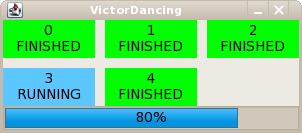
\includegraphics{images/victor_monitor}
\caption{Monitor dello stato di esecuzione del ``rendering'' di ogni gruppo di ``frame''.}
\label{fig:monitor-victor}
\end{figure}
\item Una volta che lo stato di esecuzione del ``rendering'' diventa \mgCode{FINISHED}, uscire dal programma digitando il valore $9$, seguito dal tasto \mgCode{Invio}, e, nuovamente, il valore $9$, seguito dal tasto \mgCode{Invio}.
\item All'interno della cartella da cui \mgTheApp{} \`e stato eseguito, si troveranno $5$ file in formato ZIP:
\begin{mgCodeBox}
\small
VictorDancing.blend-rendered.zip\_1\_5\newline
VictorDancing.blend-rendered.zip\_6\_10\newline
VictorDancing.blend-rendered.zip\_11\_15\newline
VictorDancing.blend-rendered.zip\_16\_20\newline
VictorDancing.blend-rendered.zip\_21\_24
\end{mgCodeBox}
\item Scompattare ciascun file all'interno di una opportuna cartella; la scompattazione creer\`a la sotto-cartella \mgCode{VictorDancing.blend-rendered} in cui si troveranno i seguenti file:
\begin{mgCodeBox}
\small
0001\_0005.avi\newline
0006\_0010.avi\newline
0011\_0015.avi\newline
0016\_0020.avi\newline
0021\_0024.avi
\end{mgCodeBox}
\item \`E ora possibile combinare i suddetti file in modo opportuno o, semplicemente, visualizzare la scena, per esempio, con il comando:
\begin{mgCodeBox}
\small
blender -a 0001\_0005.avi 0006\_0010.avi 0011\_0015.avi\newline
0016\_0020.avi 0021\_0024.avi
\end{mgCodeBox}
In Fig.~\ref{fig:exec-victor} sono mostrati alcuni fotogrammi della scena.
\end{enumerate}
Si noti che, durante l'immissione dei dati relativi alla scena, non \`e necessario inserire tutte le informazioni; in particolare, quando si accetta il valore di default proposto da \mgTheApp{} , \`e possibile evitare di accedere alla relativa voce di menu.
Ne segue che, in questo esempio, i passi descritti ai punti \ref{lbl:exec-victor-startframe-useless} e \ref{lbl:exec-victor-startframe2-useless} possono essere evitati.
Ci\`o non vale, per\`o, se la voce del menu \`e etichettata con il simbolo \mgCode{[*]} (come nel caso del file della scena), il quale indica che l'inserimento del valore \`e obbligatorio.

\begin{figure}
\centering
\begin{minipage}[t]{0.22\linewidth}
\centering
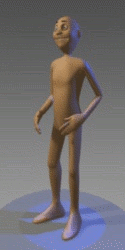
\includegraphics[scale=0.30]{images/victor-1}
\end{minipage}
\hspace{0.3cm}
\begin{minipage}[t]{0.22\linewidth}
\centering
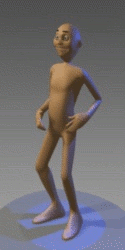
\includegraphics[scale=0.30]{images/victor-2}
\end{minipage}
\hspace{0.3cm}
\begin{minipage}[t]{0.22\linewidth}
\centering

\includegraphics[scale=0.30]{images/victor-3}
\end{minipage}
\hspace{0.3cm}
\begin{minipage}[t]{0.22\linewidth}
\centering
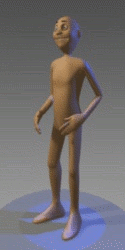
\includegraphics[scale=0.30]{images/victor-4}
\end{minipage}
\caption{Alcuni fotogrammi della scena \emph{VictorDancing}.}
\label{fig:exec-victor}
\end{figure}

\subsection{Scena: \emph{ArrayDemo}} \label{ssec:exec-arraydemo}

La scena presentata in questa sezione \`e tratta dalla sezione \emph{animation} dei test di regressione di \emph{Blender} (scena \emph{array3.blend}); l'animazione risultante, composta da $737$ ``frame'', dovrebbe rappresentare un vettore di cubi che effettuano una serie di rotazioni e traslazioni.
Il file della scena \`e presente nella sotto-cartella \mgCode{examples} della directory in cui \`e stata installata l'applicazione \mgTheApp{}.
Il ``rendering'' viene effettuato tramite una suddivisione in $30$ gruppi da $25$ ``frame'' (fatta eccezione per l'ultimo gruppo, composto da $12$ ``frame'').
A differenza della scena presentata nella sezione precedente, i file prodotti in output dal ``rendering'' di ogni gruppo di ``frame'' sono delle immagini in formato PNG.
Per ottenere il file di animazione finale, \`e necessario che nel sistema sia installato l'applicativo \emph{ffmpeg}.

Verranno ora elencati i passi per effettuare il ``rendering'' di questa scena tramite \mgTheApp{}.
\begin{enumerate}
\item Esegure l'applicazione \mgTheApp{} attraverso lo script di esecuzione \mgTheAppFile{.sh}
\begin{mgCodeBox}
\small
./\mgTheAppFile{.sh}
\end{mgCodeBox}
\item Dal menu:
\begin{mgCodeBox}
\small
\#\#\# Sharegrid Grid Renderer \#\#\#\newline
--- Main Menu:\newline
1. Insert a new job\newline
8. About\newline
9. Exit\newline
? 
\end{mgCodeBox}
Digitare il valore $1$.
\item Apparir\`a il menu che permette di inserire le informazioni sulla scena su cui effettuare il ``rendering'': digitare il valore $1$, per inserire il nome della scena, e premere il tasto \mgCode{Invio}:
\begin{mgCodeBox}
\small
\#\#\# Job selection \#\#\#\newline
--- New job\newline
1. Scene name\ \ \ \ \ \ \ \ \ \ \ \ \ \{ \}\newline
2. Scene file\ \ \ \ \ \ \ \ \ \ \ \ \ \{ \} [*]\newline
3. First frame\ \ \ \ \ \ \ \ \ \ \ \ \{ \}\newline
4. Last frame\ \ \ \ \ \ \ \ \ \ \ \ \ \{ \}\newline
5. Step frame\ \ \ \ \ \ \ \ \ \ \ \ \ \{ \}\newline
6. Input files\ \ \ \ \ \ \ \ \ \ \ \ \{ \}\newline
98. Review job settings\newline
99. Back to previous menu\newline
(---\newline
 Informations marked with:\newline
 - '[*]' are mandatory\newline
 - '\{X\}' have been already inserted by the user\newline
---)\newline
? \textbf{1}
\end{mgCodeBox}
\item Verr\`a richiesto di inserire il nome della scena; il programma offre, come valore di default, la stringa \mgCode{user-blender\_20080314\_1634}; scrivere, invece, la stringa \mgCode{ArrayDemo} e premere il tasto \mgCode{Invio}:
\begin{mgCodeBox}
\small
\{Scene name>> Symbolic name used for identifying the scene [user-blender\_20080314\_1634]? \textbf{ArrayDemo}
\end{mgCodeBox}
\item Apparir\`a nuovamente il menu relativo ai dati della scena; digitare il valore $2$, per inserire il percorso al file della scena, e premere il tasto \mgCode{Invio}:
\begin{mgCodeBox}
\small
\#\#\# Job selection \#\#\#\newline
--- New job\newline
1. Scene name\ \ \ \ \ \ \ \ \ \ \ \ \ \{X\}\newline
2. Scene file\ \ \ \ \ \ \ \ \ \ \ \ \ \{ \} [*]\newline
3. First frame\ \ \ \ \ \ \ \ \ \ \ \ \{ \}\newline
4. Last frame\ \ \ \ \ \ \ \ \ \ \ \ \ \{ \}\newline
5. Step frame\ \ \ \ \ \ \ \ \ \ \ \ \ \{ \}\newline
6. Input files\ \ \ \ \ \ \ \ \ \ \ \ \{ \}\newline
98. Review job settings\newline
99. Back to previous menu\newline
(---\newline
 Informations marked with:\newline
 - '[*]' are mandatory\newline
 - '\{X\}' have been already inserted by the user\newline
---)\newline
? \textbf{2}
\end{mgCodeBox}
\item Verr\`a richiesto di inserire il percorso al file della scena; il programma offre, come valore di default il file \mgCode{user-blender\_20080314\_1634}; scrivere, invece, la stringa \mgCode{./examples/data/blender/array3.blend} e premere il tasto \mgCode{Invio}:
\begin{mgCodeBox}
\small
\{Scene file>> Path to the scene file [user-blender\_20080314\newline
\_1634.blend]?  \textbf{./examples/data/blender/array3.blend}
\end{mgCodeBox}
\item \label{lbl:exec-array3-startframe-useless} Apparir\`a nuovamente il menu relativo ai dati della scena; digitare il valore $3$, per inserire il numero del primo ``frame'' da sottoporre al ``rendering'', e premere il tasto \mgCode{Invio}:
\begin{mgCodeBox}
\small
\#\#\# Job selection \#\#\#\newline
--- New job\newline
1. Scene name\ \ \ \ \ \ \ \ \ \ \ \ \ \{X\}\newline
2. Scene file\ \ \ \ \ \ \ \ \ \ \ \ \ \{X\} [*]\newline
3. First frame\ \ \ \ \ \ \ \ \ \ \ \ \{ \}\newline
4. Last frame\ \ \ \ \ \ \ \ \ \ \ \ \ \{ \}\newline
5. Step frame\ \ \ \ \ \ \ \ \ \ \ \ \ \{ \}\newline
6. Input files\ \ \ \ \ \ \ \ \ \ \ \ \{ \}\newline
98. Review job settings\newline
99. Back to previous menu\newline
(---\newline
 Informations marked with:\newline
 - '[*]' are mandatory\newline
 - '\{X\}' have been already inserted by the user\newline
---)\newline
? \textbf{3}
\end{mgCodeBox}
\item \label{lbl:exec-array3-startframe2-useless} Verr\`a richiesto di inserire il numero del primo ``frame'' da cui iniziare il ``rendering'' della scena; il programma offre, come valore di default il valore $1$; accettare tale valore premendo il tasto \mgCode{Invio} (senza immettere alcun valore):
\begin{mgCodeBox}
\small
\{Start frame>> Number of the first frame of the scene to be rendered [1]?
\end{mgCodeBox}
\item Apparir\`a nuovamente il menu relativo ai dati della scena; digitare il valore $4$, per inserire il numero dell'ultimo ``frame'' da sottoporre al ``rendering'', e premere il tasto \mgCode{Invio}:
\begin{mgCodeBox}
\small
\#\#\# Job selection \#\#\#\newline
--- New job\newline
1. Scene name\ \ \ \ \ \ \ \ \ \ \ \ \ \{X\}\newline
2. Scene file\ \ \ \ \ \ \ \ \ \ \ \ \ \{X\} [*]\newline
3. First frame\ \ \ \ \ \ \ \ \ \ \ \ \{X\}\newline
4. Last frame\ \ \ \ \ \ \ \ \ \ \ \ \ \{ \}\newline
5. Step frame\ \ \ \ \ \ \ \ \ \ \ \ \ \{ \}\newline
6. Input files\ \ \ \ \ \ \ \ \ \ \ \ \{ \}\newline
98. Review job settings\newline
99. Back to previous menu\newline
(---\newline
 Informations marked with:\newline
 - '[*]' are mandatory\newline
 - '\{X\}' have been already inserted by the user\newline
---)\newline
? \textbf{4}
\end{mgCodeBox}
\item Verr\`a richiesto di inserire il numero dell'ultimo ``frame'' in cui terminare il ``rendering'' della scena; il programma offre, come valore di default il valore assunto dal primo ``frame'', in questo caso il valore $1$; digitare il valore $737$ e premere il tasto \mgCode{Invio}:
\begin{mgCodeBox}
\small
\{End frame>> Number of the last frame of the scene to be rendered [1]? \textbf{737}
\end{mgCodeBox}
\item \label{lbl:exec-array3-stepframe-useless} Apparir\`a nuovamente il menu relativo ai dati della scena; digitare il valore $5$, per inserire il numero di ``frame'' da includere in ciascun gruppo, e premere il tasto \mgCode{Invio}:
\begin{mgCodeBox}
\small
\#\#\# Job selection \#\#\#\newline
--- New job\newline
1. Scene name\ \ \ \ \ \ \ \ \ \ \ \ \ \{X\}\newline
2. Scene file\ \ \ \ \ \ \ \ \ \ \ \ \ \{X\} [*]\newline
3. First frame\ \ \ \ \ \ \ \ \ \ \ \ \{X\}\newline
4. Last frame\ \ \ \ \ \ \ \ \ \ \ \ \ \{X\}\newline
5. Step frame\ \ \ \ \ \ \ \ \ \ \ \ \ \{ \}\newline
6. Input files\ \ \ \ \ \ \ \ \ \ \ \ \{ \}\newline
98. Review job settings\newline
99. Back to previous menu\newline
(---\newline
 Informations marked with:\newline
 - '[*]' are mandatory\newline
 - '\{X\}' have been already inserted by the user\newline
---)\newline
? \textbf{5}
\end{mgCodeBox}
\item \label{lbl:exec-array3-stepframe2-useless} Verr\`a richiesto di inserire il numero di ``frame'' da includere in ciascuna partizione della scena; il programma offre, come valore di default il valore $25$; accettare tale valore premendo il tasto \mgCode{Invio} (senza immettere alcun valore):
\begin{mgCodeBox}
\small
\{Step frame>> Number of contiguous frames the scene will be subdivided [25]?
\end{mgCodeBox}
\item Apparir\`a nuovamente il menu relativo ai dati della scena; dato che la scena non necessita di ulteriori risorse addizionali, la voce numero $6$ del menu verr\`a saltata. Digitare il valore $98$, per visualizzare il riepilogo delle informazioni inserire, e premere il tasto \mgCode{Invio}:
\begin{mgCodeBox}
\small
\#\#\# Job selection \#\#\#\newline
--- New job\newline
1. Scene name\ \ \ \ \ \ \ \ \ \ \ \ \ \{X\}\newline
2. Scene file\ \ \ \ \ \ \ \ \ \ \ \ \ \{X\} [*]\newline
3. First frame\ \ \ \ \ \ \ \ \ \ \ \ \{X\}\newline
4. Last frame\ \ \ \ \ \ \ \ \ \ \ \ \ \{X\}\newline
5. Step frame\ \ \ \ \ \ \ \ \ \ \ \ \ \{X\}\newline
6. Input files\ \ \ \ \ \ \ \ \ \ \ \ \{ \}\newline
98. Review job settings\newline
99. Back to previous menu\newline
(---\newline
 Informations marked with:\newline
 - '[*]' are mandatory\newline
 - '\{X\}' have been already inserted by the user\newline
---)\newline
? \textbf{98}
\end{mgCodeBox}
\item Verranno visualizzate le seguenti informazioni:
\begin{mgCodeBox}
\small
Scene name: ArrayDemo\newline
Scene file: ./examples/data/blender/array3.blend\newline
Start frame number: 1\newline
End frame number: 737\newline
Step frame number: 25\newline
Input files:  <none>\newline
\end{mgCodeBox}
\item Apparir\`a nuovamente il menu relativo ai dati della scena. Digitare il valore $99$, per ritornare al menu principale, e premere il tasto \mgCode{Invio}:
\begin{mgCodeBox}
\small
\#\#\# Job selection \#\#\#\newline
--- New job\newline
1. Scene name\ \ \ \ \ \ \ \ \ \ \ \ \ \{X\}\newline
2. Scene file\ \ \ \ \ \ \ \ \ \ \ \ \ \{X\} [*]\newline
3. First frame\ \ \ \ \ \ \ \ \ \ \ \ \{X\}\newline
4. Last frame\ \ \ \ \ \ \ \ \ \ \ \ \ \{X\}\newline
5. Step frame\ \ \ \ \ \ \ \ \ \ \ \ \ \{X\}\newline
6. Input files\ \ \ \ \ \ \ \ \ \ \ \ \{ \}\newline
98. Review job settings\newline
99. Back to previous menu\newline
(---\newline
 Informations marked with:\newline
 - '[*]' are mandatory\newline
 - '\{X\}' have been already inserted by the user\newline
---)\newline
? \textbf{99}
\end{mgCodeBox}
\item Apparir\`a il menu iniziale, arricchito di nuove informazioni; a questo punto \`e possibile ritornare al menu dei dati della scena per modificare le informazioni appena inserite (voce numero $2$ del menu), eseguire il ``rendering'' distribuito della scena (voce numero $3$ del menu), esportare su un file i dati appena inseriti (voce numero $4$ del menu) oppure inserire una nuova scena, sostituiendo i dati appena inseriti (voce del menu $1$).
Supponendo di voler lanciare il ``rendering'' della scena, digitare il valore $3$ e premere il tasto \mgCode{Invio}:
\begin{mgCodeBox}
\small
\#\#\# Sharegrid Grid Renderer \#\#\#\newline
--- Main Menu:\newline
1. Insert a new job\newline
2. Modify current job\newline
3. Execute current job\newline
4. Export current job\newline
8. About\newline
9. Exit\newline
? \textbf{3}
\end{mgCodeBox}
\item L'applicazione \mgTheApp{} contatter\`a lo ``scheduler'' \emph{mygrid}.
\begin{itemize}
\item Se l'interazione con ``mygrid'' ha successo verr\`a visualizzato il messaggio di conferma:
\begin{mgCodeBox} 
\small
\textcolor{green}{[OK] Job successfully submitted.}\newline
\textcolor{blue}{[INFO] The job execution identifier is: 2}\newline
\textcolor{blue}{[INFO] Use this identifier for retrieving job\newline
execution information or for cancelling the job\newline
execution.}
\end{mgCodeBox} 
\item Se ``mygrid'' non \`e in esecuzione verr\`a visualizzato il messaggio di errore:
\begin{mgCodeBox}
\small
\textcolor{red}{[ERROR] Current job cannot be executed. Please, check if the scheduler is running!}
\end{mgCodeBox}
Per risolvere il problema, \`e sufficiente eseguire l'applicazione \emph{mygrid} (non \`e necessario uscire dall'applicazione \mgTheApp{}) e digitare nuovamente il valore $3$ per tentare l'esecuzione.
\end{itemize}
\item Il valore indicato come \emph{job execution identifier}, restituito quando \mgTheApp{} riesce a sottomettere con successo, a \emph{mygrid}, le istruzioni per il ``rendering'', pu\`o essere utilizzato sia all'interno di \mgTheApp{} per ottenere informazioni sullo stato di esecuzione o per annullare l'esecuzione, sia attraverso l'interfaccia testuale o grafica di \emph{mygrid}. Per esempio, per visualizzare lo stato di esecuzione, digitare il valore $1$ e premere il tasto \mgCode{Invio}:
\begin{mgCodeBox}
\small
\#\#\# Job execution \#\#\#\newline
1. Execution status\newline
2. Cancel execution\newline
3. Execute again\newline
4. Monitor execution\newline
9. Back to previous menu\newline
? \textbf{1}
\end{mgCodeBox}
\item Verr\`a visualizzato un messaggio indicante lo stato di esecuzione del ``rendering''; per esempio, il messaggio:
\begin{mgCodeBox}
\small
\textcolor{blue}{[INFO] The execution IDENTIFIER of the job is: 2}\newline
\textcolor{blue}{[INFO] The execution STATUS of the job is: RUNNING}
\end{mgCodeBox}
informa che il ``rendering'', con ``job execution identifier'' pari a $1$, \`e attualmente in esecuzione (\mgCode{RUNNING}).
\item \`E inoltre possibile osservare lo stato di esecuzione del job in modo interattivo attraverso un'interfaccia grafica; per eseguire tale interfaccia, digitare il valore $4$ e premere il tasto \mgCode{Invio}:
\begin{mgCodeBox}
\small
\#\#\# Job execution \#\#\#\newline
1. Execution status\newline
2. Cancel execution\newline
3. Execute again\newline
4. Monitor execution\newline
9. Back to previous menu\newline
? \textbf{4}
\end{mgCodeBox}
\item Verr\`a visualizzato un messaggio di conferma di esecuzione del monitor di job:
\begin{mgCodeBox}
\small
\textcolor{green}{[OK] Job monitor has been successfully started.}
\end{mgCodeBox}
e apparir\`a una finestra indicante lo stato di esecuzione del ``rendering'' di ogni gruppo di ``frame'' in cui il ``rendering'' dell'intera scena \`e stato scomposto (Fig.~\ref{fig:monitor-arraydemo}).
\begin{figure}
\centering
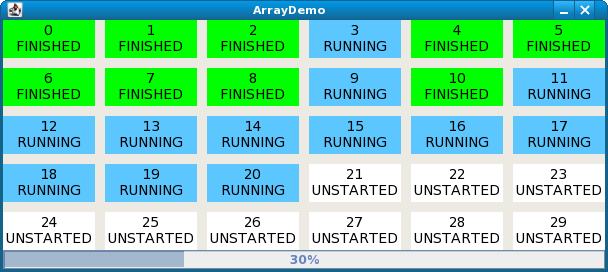
\includegraphics{images/array3_monitor}
\caption{Monitor dello stato di esecuzione del ``rendering'' di ogni gruppo di ``frame''.}
\label{fig:monitor-arraydemo}
\end{figure}
\item \label{lbl:exec-array3-postrenderstep1} Una volta che lo stato di esecuzione del ``rendering'' diventa \mgCode{FINISHED}, uscire dal programma digitando il valore $9$, seguito dal tasto \mgCode{Invio}, e, nuovamente, il valore $9$, seguito dal tasto \mgCode{Invio}.
\item \label{lbl:exec-array3-postrenderstep2} All'interno della cartella da cui \mgTheApp{} \`e stato eseguito, si troveranno $30$ file in formato ZIP:
\begin{mgCodeBox}
\small
array3.blend-rendered.zip\_1\_25\newline
array3.blend-rendered.zip\_26\_50\newline
array3.blend-rendered.zip\_51\_75\newline
array3.blend-rendered.zip\_76\_100\newline
array3.blend-rendered.zip\_101\_125\newline
array3.blend-rendered.zip\_126\_150\newline
array3.blend-rendered.zip\_151\_175\newline
array3.blend-rendered.zip\_176\_200\newline
array3.blend-rendered.zip\_201\_225\newline
array3.blend-rendered.zip\_226\_250\newline
array3.blend-rendered.zip\_251\_275\newline
array3.blend-rendered.zip\_276\_300\newline
array3.blend-rendered.zip\_301\_325\newline
array3.blend-rendered.zip\_326\_350\newline
array3.blend-rendered.zip\_351\_375\newline
array3.blend-rendered.zip\_376\_400\newline
array3.blend-rendered.zip\_401\_425\newline
array3.blend-rendered.zip\_426\_450\newline
array3.blend-rendered.zip\_451\_475\newline
array3.blend-rendered.zip\_476\_500\newline
array3.blend-rendered.zip\_501\_525\newline
array3.blend-rendered.zip\_526\_550\newline
array3.blend-rendered.zip\_551\_575\newline
array3.blend-rendered.zip\_576\_600\newline
array3.blend-rendered.zip\_601\_625\newline
array3.blend-rendered.zip\_626\_650\newline
array3.blend-rendered.zip\_651\_675\newline
array3.blend-rendered.zip\_676\_700\newline
array3.blend-rendered.zip\_701\_725\newline
array3.blend-rendered.zip\_726\_737
\end{mgCodeBox}
\item \label{lbl:exec-array3-postrenderstep3} Scompattare ciascun file all'interno di una opportuna cartella; la scompattazione creer\`a la sotto-cartella \mgCode{array3.blend-rendered} in cui si troveranno i seguenti file:
\begin{mgCodeBox}
\small
0001.png\newline
0002.png\newline
\dots\newline
0737.png
\end{mgCodeBox}
\item \label{lbl:exec-array3-postrenderstep4} \`E ora possibile combinare i suddetti file in modo opportuno, per esempio con il comando:
\begin{mgCodeBox}
\small
ffmpeg -i \%04d.png array3.mpeg
\end{mgCodeBox}
In Fig.~\ref{fig:exec-array3} sono mostrati alcuni fotogrammi della scena.
\begin{figure}
\centering
\begin{tabular}{ccc}
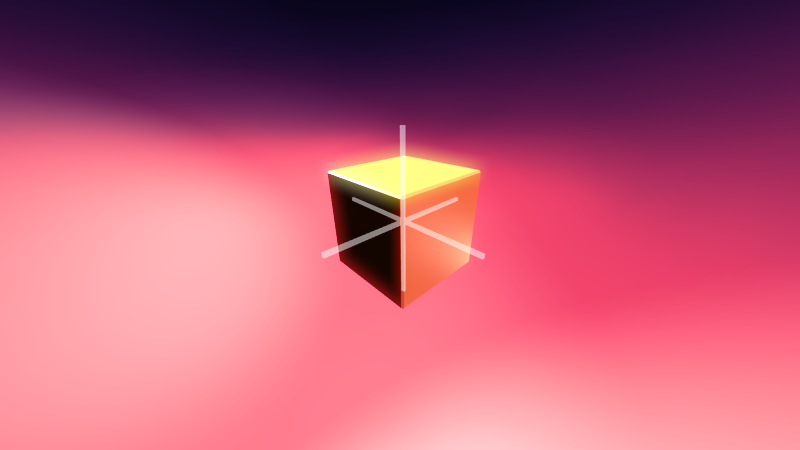
\includegraphics[scale=0.17]{images/array3-1} &
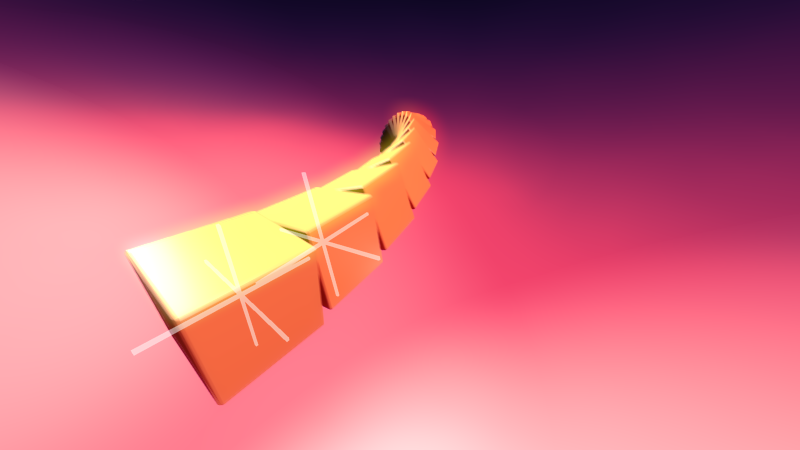
\includegraphics[scale=0.17]{images/array3-2} &
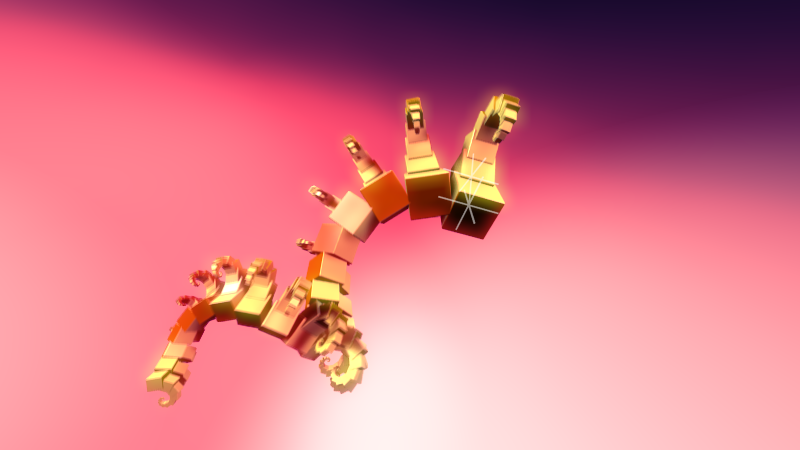
\includegraphics[scale=0.17]{images/array3-3} \tabularnewline
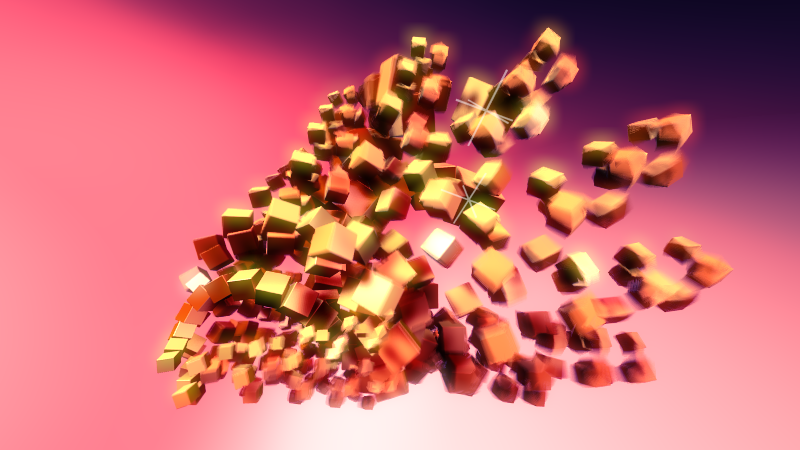
\includegraphics[scale=0.17]{images/array3-4} &
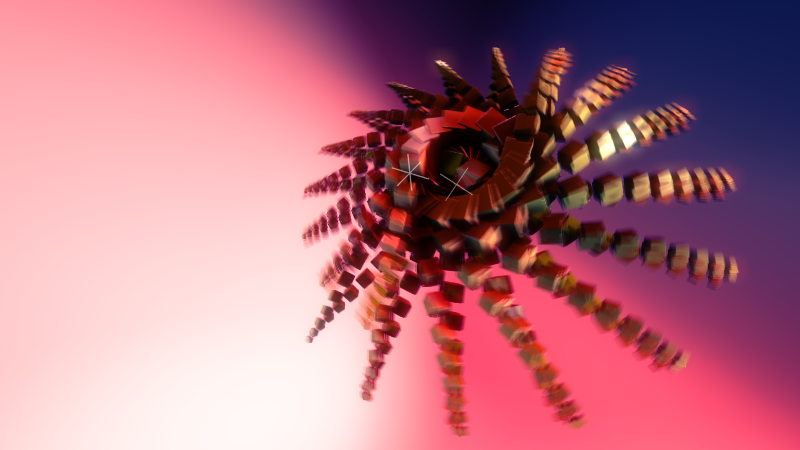
\includegraphics[scale=0.17]{images/array3-5} &
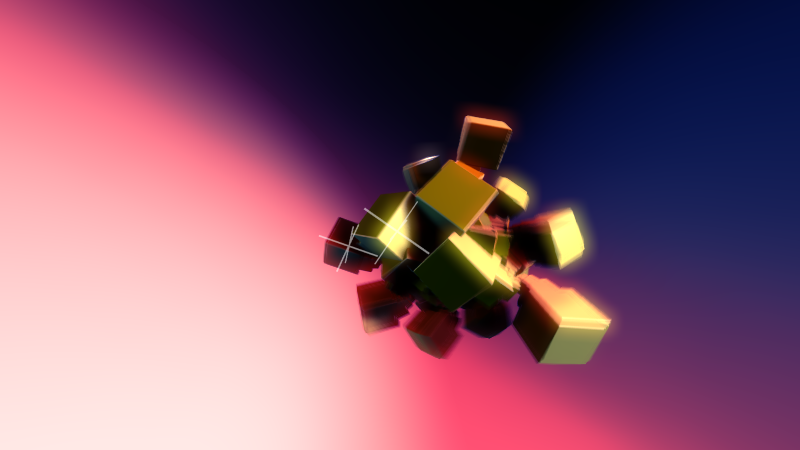
\includegraphics[scale=0.17]{images/array3-6} \tabularnewline
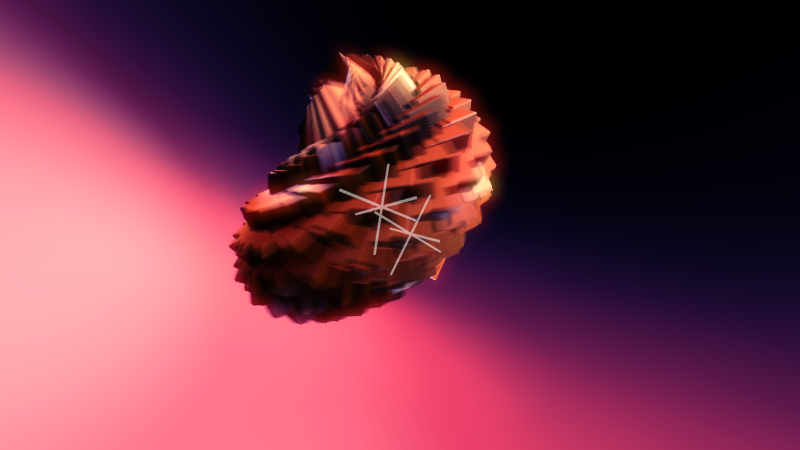
\includegraphics[scale=0.17]{images/array3-7} &
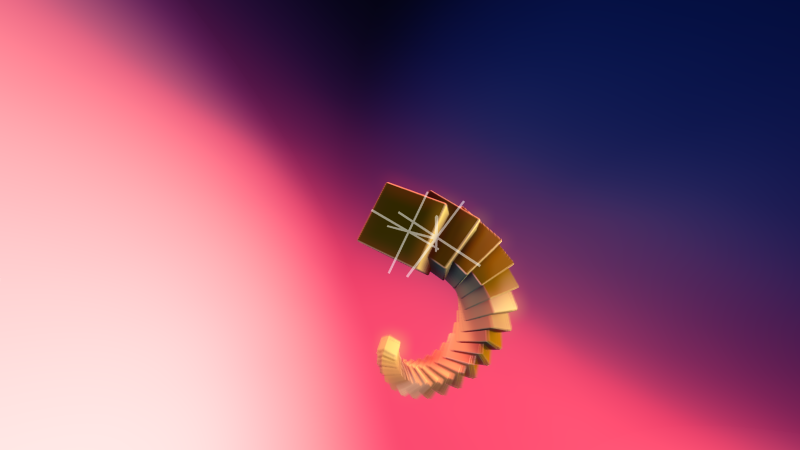
\includegraphics[scale=0.17]{images/array3-8} &
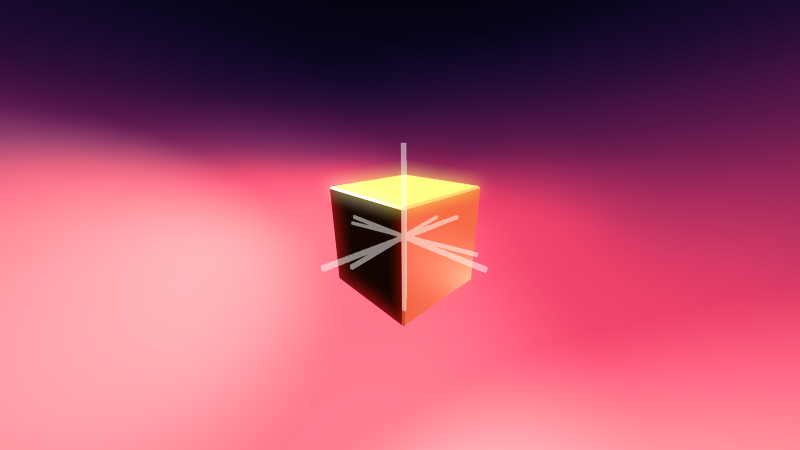
\includegraphics[scale=0.17]{images/array3-9}
\end{tabular}
\caption{Alcuni fotogrammi della scena \emph{ArrayDemo}.}
\label{fig:exec-array3}
\end{figure}
\end{enumerate}
Si noti che, durante l'immissione dei dati relativi alla scena, non \`e necessario inserire tutte le informazioni; in particolare, quando si accetta il valore di default proposto da \mgTheApp{} , \`e possibile evitare di accedere alla relativa voce di menu.
Ne segue che, in questo esempio, i passi descritti ai punti \ref{lbl:exec-array3-startframe-useless}, \ref{lbl:exec-array3-startframe2-useless}, \ref{lbl:exec-array3-stepframe-useless} e \ref{lbl:exec-array3-stepframe2-useless} possono essere evitati.
Ci\`o non vale, per\`o, se la voce del menu \`e etichettata con il simbolo \mgCode{[*]} (come nel caso del file della scena), il quale indica che l'inserimento del valore \`e obbligatorio.

I passi \ref{lbl:exec-array3-postrenderstep1}, \ref{lbl:exec-array3-postrenderstep2}, \ref{lbl:exec-array3-postrenderstep3} e \ref{lbl:exec-array3-postrenderstep4} possono essere automatizzati eseguendo lo script \emph{images2movie.sh}:
\begin{mgCodeBox}
./images2movie.sh array3 png
\end{mgCodeBox}
dove il primo argomento (in questo caso \emph{array3}) rappresenta il nome del file della scena (senza l'estensione \emph{.blend}), mentre il secondo argomento (in questo caso \emph{png}) rappresenta il formato delle immagini prodotte dal ``rendering'' dei vari gruppi di ``frame''.
L'uso di questo script necessita che nel sistema siano installati gli applicativi \emph{ffmpeg} e \emph{ffplay}.


%%%%%%%%%%%%%%%%%%%%%%%%%%%%%%%%%%%%%%%%%%%%%%%%%%%%%%%%%%%%%%%%%%%%%%%%%%%%%%%%

%%@{ bibliography

%\nocite{*}

\bibliography{UserGuide}

%%@} bibliography

\end{document}

%%@} document body
